\chapter{Raft Consensus Algorithm}

The previous chapters introduced the problem of consensus and explained why Raft has become the go-to solution. This chapter acts as an introduction to Raft, based on Diego Ongaro's PhD dissertation \cite{raft}, but does not provide a complete specification of the algorithm. The reader is rather encouraged to look into the dissertation for further details. Additionally, Chapter 3 will also touch on some key details that have been left out when describing this paper's implementation of Raft.

\section{Overview}

Raft's purpose is to maintain a replicated state machine across a cluster of servers.\\

First, a state machine needs to be defined and hosted in all servers of the cluster. The definition is specific to each use-case, but it must always describe a deterministic state machine. Deterministic state machines require that given the same initial state and the same sequence of commands, the state machine will always reach the same final state.\\

Raft then accepts a sequence of commands from clients, called the log, and sends them in order to all servers. This process is called "log replication", and it also involves the resolution of conflicts that may occur. The servers store the log in their own private storage and apply the commands to their state machines when instructed.\\

In the end, the same sequence of commands will have been applied to the state machines in all participating servers. Since these state machines are deterministic, they will all have reached the same final state; thus, the state machine will have been replicated.\\

\section{Raft Cluster and Server States}

Raft splits time into distinct periods called terms and assigns one of three roles to each server in every term. The roles are: Leader, Candidate, and Follower.

\subsection{Terms as a Logical Clock}

The term is a monotonically increasing integer that marks a section of time, but it does not correspond to any specific time interval. Rather, it acts as a logical clock \cite{logical-clocks}. Each term begins with an election, where one or more servers, acting as candidates, attempt to become the leader. One of the candidates is selected and acts as the leader for the remainder of the term. A term ends when any server detects that the current leader is no longer viable, triggering a new election for a new term. Note that Raft guarantees that only a single server will act as the leader for a term.\\

Each server stores the current term and includes it in any messages it sends to other servers. All servers validate incoming messages by comparing the contained term with their own; any messages from older terms are rejected. This is an essential component of Raft's safety guarantees, as it prevents servers with a stale snapshot of the log from erroneously modifying the replicated state machine.\\

\subsection{Leader}

When a node is elected as the leader, it becomes responsible for managing the replicated state machine. Any commands from clients are directed to the leader, which validates and applies them. The leader also instructs followers to apply the received commands to their internal state machines, which are then marked as committed.\\

A leader is expected to periodically inform other servers that it is still viable by sending heartbeat messages. When a leader fails and is unable to progress the replicated state machine, it also becomes unable to send these heartbeats. Then, after a specified time interval passes, called the election timeout, other servers detect that the leader is not viable anymore and will attempt to elect a new one.\\

Any leader may became non-operational for a time period and later rejoin the cluster. In that case, it will receive heartbeats from the new leader and revert to a follower state.

\subsection{Candidate}

When a follower has not received valid heartbeats for a period exceeding the election timeout, it attempts to elect itself as the leader. The server begins an election for a new term by acting as a candidate, implicitly voting for itself, and soliciting votes from the rest of the servers. When a server succeeds in becoming the leader, it starts sending heartbeats to the rest of the cluster, informing them of its victory. A candidate will revert to follower if it detects another server that managed to become a leader for the term instead.\\

Ties in the leader election process are made rare by using a dynamic interval for the election timeout. At the beginning of a term, each server picks a random interval within a specified range and uses that as its election timeout. Thus, most often there will be a single candidate who got a head start in soliciting votes, minimizing the probability of ties.\\

\subsection{Follower}

Followers are passive members of the cluster. They receive commands from the leader and apply them to their local state machines. Followers also participate in the election process by responding to vote requests from candidates or by becoming candidates themselves after an election timeout.

\begin{figure}[ht]
  \centering
  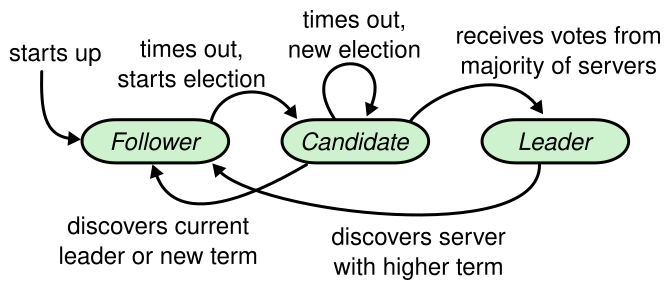
\includegraphics[width=400pt]{images/followercandidateleader.png}
  \caption{High level overview of the different server states and the transitions between them. It is taken from Diego Ongaro's PhD dissertation \cite{raft}.}
  \label{fig:raft-states-transitions}
\end{figure}

\section{Raft Properties} \label{raft-properties}

One of the reasons Raft has become so prevalent is the guarantees it carries about its behavior. Namely, Raft guarantees the following properties: Election Safety, Leader Append-Only, Log Matching, Leader Completeness, State Machine Safety \cite{raft}. They are essential in keeping Raft implementations simple, since developers can easily reason about the system's behavior. They are also formally proven \cite{raft} and can be trusted to always hold.\\

Each property is briefly described as follows:
\begin{itemize}
    \item \textbf{Election Safety}: At any given term, only one server will be acting as the leader. The leader is responsible for advancing the replicated state machine and needs to do so without conflict.
    \item \textbf{Leader Append-Only}: A server, when acting as the leader, can append commands to its internal log but never overwrite or delete previous commands. This is an essential building block for providing the final three properties.
    \item \textbf{Log Matching}: When the logs of two servers contain a command with the same index that was created in the same term, it is guaranteed that all commands up to and including this command are completely identical in their contents.
    \item \textbf{Leader Completeness}: A command that is successfully committed in a term will always be present in the logs of all subsequent leaders.
    \item \textbf{State Machine Safety}: When a server is instructed to apply a command at a certain index to its state machine, it is guaranteed that no other server will apply a different command at the same index to its own state machine.
\end{itemize}

\section{Fault Tolerance in Raft}

As stated before, Raft is particularly appealing because it can continue advancing the replicated state machine in the face of failures, while not sacrificing its strong consistency guarantees. Specifically, any minority of servers can become in some way non-operational without impeding progress. \\

To make this fact apparent, the exact conditions under which the leader election and log replication processes succeed are presented below.

\subsection{Leader Election} \label{leader-election-fault-tolerance}

During an election cycle, a candidate only needs to gather votes from the majority of the cluster before declaring itself the leader for the term and sending heartbeats to all other servers. Notably, it is possible for multiple servers to become candidates and attempt to solicit votes simultaneously, but at most one of them can succeed. This is ensured by restricting each server to vote for only a single candidate in each term. At worst, none the candidates will receive a majority of votes, resulting in a tie. In that case, after an election timeout, they will attempt to get elected for the next term. Note that each server's vote for each term is made durable by persisting it along with the log, enabling it to survive restarts and other failures.\\

\subsection{Log Replication}

During log replication, a command is considered successfully replicated, or committed, once a majority of the cluster has received and stored it. Then, the command will take effect and will be visible to clients.\\

Raft can guarantee that the internal log of any elected leader will contain all commands committed by previous leaders, even without requiring successful replication to all servers. This is implemented by applying an additional rule during leader election; a voter will reject a candidate if the candidate's log is less up to date than its own. Having this guarantee, newly elected leaders can immediately start accepting requests from clients and further advancing the log safely.\\

Further, it is not possible for a leader that was for a time period not operational to later rejoin the cluster and erroneously modify the replicated log. This is implemented via a restriction during log replication. Leaders attempting to replicate commands include their current term in their requests to followers. A leader that has lost its authority in the cluster will use a stale term, prompting other servers to reject its requests and forcing it to become a follower.\\

\subsection{Failure Types}

At this point, the specific types of failures that Raft can handle should be noted; Raft assumes that a failing server is either unable to function or unable to communicate with other servers.\\

A Raft server can be unable to function due to power loss, hardware failure, or other exceptional conditions that interrupt its runtime. Failing servers will be unable to respond to any requests, either from clients or from other servers.\\

A Raft server can become unable to communicate due to failures in the network infrastructure connecting the cluster, resulting in a network partition. Partitioned servers will look identical to failing servers to the rest of the cluster but, importantly, will still seem operational to servers and clients on the same side of the partition. This characteristic of partitions makes them uniquely dangerous for consensus mechanisms due to their potential for causing split-brains. This will be discussed further in subsection \ref{split-brains}.\\

Raft can tolerate both of these cases as long as there is still a majority of operational servers that can communicate. Notably, Raft cannot cope with servers that fail by exhibiting arbitrary or malicious behavior. Such conditions are called Byzantine faults in the literature and there have been efforts to describe a version of Raft that can effectively guard against them \cite{tian2021byzantine,xie2022raft,zhou2021vg,copeland2016tangaroa}. \\

\subsection{Guarding Against the Split-Brain Problem} \label{split-brains}

As mentioned previously, network partitions give rise to the unique problem of split-brains in consensus mechanisms. A cluster of servers enters a split-brain condition when groups of servers are isolated from each other, resulting in the erroneous formation of multiple independent clusters.\\

Raft in its original form can effectively prevent split-brains without modification; the described log replication and leader election processes can only succeed if a majority of the cluster can communicate. If a cluster gets partitioned, there will be at most one majority formed, which can continue advancing the log safely. If the cluster is partitioned in a way that does not allow for any majority to form, the cluster will become unable to fulfill client requests until the partition is resolved.\\

However, Raft is susceptible to split-brains when the cluster supports dynamic reconfigurations, even in the absence of partitions. Dynamic cluster reconfiguration refers to the addition or removal of servers from the cluster without any interruption of service. If multiple servers are added at once, a window of time is created where separate majorities can form \cite{raft}, as demonstrated by Figure \ref{fig:reconfiguration-difficulty}.\\ 

Permitting only a single server addition at a time will eliminate such cases as it can never result in the formation of separate majorities \cite{raft}. More servers can be added once the previous server addition has been acknowledged by the entirety of the cluster. Additionally, Raft provides a solution for "Arbitrary configuration changes using joint consensus" \cite{raft}. Although this solution can allow more than one server to be added at a time, it is complex and not essential for most real-world applications.


\begin{figure}[ht]
  \centering
  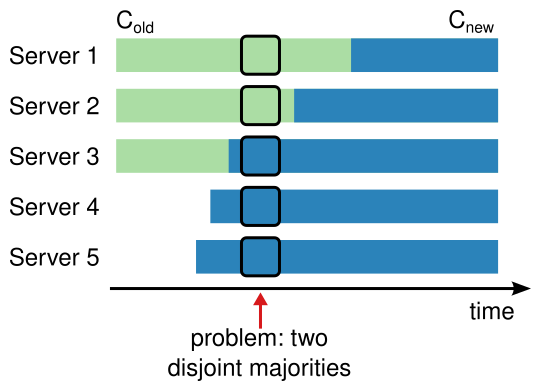
\includegraphics[width=400pt]{images/reconfigurationdifficulty.png}
  \caption{The transition from the old configuration ($C_{old}$) of three servers to the new configuration ($C_{new}$) of five servers happens incrementally and different servers observe it at different times. In this case, there is a period in time where $Server_1$, $Server_2$, and $Server_3$ can form one majority, while $Server_3$, $Server_4$, and $Server_5$ can form another. This figure is taken from Diego Ongaro's PhD dissertation \cite{raft}.}
  \label{fig:reconfiguration-difficulty}
\end{figure}

\section{Scalability concerns in Raft} \label{scalabilirt-raft-multi-raft}

In Raft, larger cluster sizes provide additional fault tolerance, since more servers can become non-operational while still keeping a majority alive. However, a Raft cluster does not improve its performance by using the computational resources of additional servers. At any given point in time, only the leader is performing meaningful work, and other servers act as replicas, ready to take the reigns when the leader fails. In fact, as cluster sizes increase, Raft's processes incur additional overhead, since they require performing broadcast requests to increasingly more servers. 

\subsection{Raft Cluster Sizing}

These performance considerations have generally led to the recommendation that Raft clusters comprise of three, five, or seven servers.\\ 

Three servers is the minimum, as any smaller size provides no fault tolerance. Seven is thought to be a sensible maximum, since it provides enough fault tolerance in real-world use cases while not incurring significant overhead. Clusters of four or six servers, while viable, are not encouraged. These sizes carry the same fault tolerance characteristics of clusters with one less server, incurring needless overhead. To demonstrate this, consider that in clusters of both three and four servers, only a single server can fail, as the majority in the first case requires two, and in the second case three servers. The same is true for clusters of five and six servers; in both cases, at most two servers can fault.\\

\subsection{Increased Scalability with Multi-Raft}

A successful method for achieving higher scalability with Raft has been to segment the replicated state machine into multiple parts, running an independent Raft process for each of them. Incoming client requests are deterministically routed to a single one of these processes, effectively implementing a sharded architecture \cite{solat2024sharding}.
Such a setup has typically been called Multi-Raft and is common in distributed databases that use Raft, such as CockroachDB \cite{cockroachDb-multi-raft}.\\

In the simplest case, all servers in the cluster run one Raft process per state machine. Different servers can then be elected as leaders for each of the independent Raft processes, thus spreading the load. Usually, mechanisms need to be put in place for preventing single servers from becoming the leader for a disproportionately large share of state machines. Additionally, messages generated by each Raft process are usually grouped and sent in batches to other servers, mitigating the increase in message volume caused by the multiple Raft instances.\\

Although the described design spreads the load within a cluster more evenly, it does not enable larger cluster sizes. To achieve that, implementations can restrict the number of servers participating in each of the Raft processes. For example, a cluster of fifteen servers can be used, with each of the processes hosted in overlapping groups of five. In such setups, additional mechanisms need to be put in place for assigning each Raft process to specific servers and for routing client requests to them.\\

\subsection{Utilizing Followers for Reads}

Notably, it is possible for a Raft cluster to utilize follower servers for fulfilling some types of requests, spreading the load somewhat without Multi-Raft.\\

A follower can use its internal log to reply to clients seeking to simply read the current state of the state machine. However, the follower's log may be stale, as the leader might not have replicated a committed command to it yet. Implementations can choose to accept the possibility of staleness, or instruct the follower to first verify that its log is up to date before replying.\\